\documentclass[14pt,fleqn]{article}
\usepackage[russian]{babel}
\usepackage{amssymb}
\usepackage{graphicx}
\usepackage{mathtools}
\usepackage{listings}
\usepackage{enumerate}
\usepackage{systeme}
\usepackage{comment}
\usepackage{xcolor}
\usepackage{geometry}
\DeclarePairedDelimiter{\floor}{\lfloor}{\rfloor}
\DeclarePairedDelimiter{\ceil}{\lceil}{\rceil}
\geometry{
	a4paper,
	total={170mm,257mm},
	left=20mm,
	top=20mm,
}
\setlength\mathindent{0pt}

\newenvironment{amatrix}[1]{%
	\left(\begin{array}{@{}*{#1}{c}|c@{}}
	}{%
	\end{array}\right)
}

\renewcommand{\mod}{\text{ mod }}

\newcommand{\DFT}{\text{DFT}}

\title{Метапрограммирование, домашнее задание 1, кейс 2.}
\author{Васильев Даниил Алексеевич, БПМИ-193-2}
\date{}

\begin{document}
\maketitle

\large{
\begin{itemize}
\item Ситуация: Сохранённые миры на разных платформах располагаются в разных папках и имеют разные расширения. Мы уже умеем переводить мир в строку для сохранения в файл.
\item Задача: Нужно написать модуль, который в соответствии с платформой сохраняет конвертированный в строку мир куда надо и в определённом расширении файла.
\item Решение: Перефразируя задачу, нужно неявно конвертировать строку в файл. Это собственно делает адаптер.

Проблема возникает в том, что платформ много и они могут сильно различаться. Нам нельзя сделать "универсальный" адаптер, т.к. это нарушает ISP.

Тогда на каждую платформу придётся писать отдельный адаптер. Предположим, что мы решили не делать один адаптер-интерфейс, и каждый адаптер никак не связан с другими. По SRP понятно, что мы отделили эту задачу от других модулей. То есть адаптер использует другой класс. Тогда, т.к. адаптеры не связаны интерфейсом, то придётся делать копии использующего класса на каждый адаптер, что нарушает DRY.

Тогда нам придётся сделать интерфейс-адаптер и вставлять туда конкретную реализацию адаптера. Иными словами, мы только что воспользовались фабричным методом для создания адаптеров.

\item Объясню UML-диаграмму, указанную на странице ниже: Пусть клиент передаёт мир как строку в отдельный класс WorldSaver и хочет, чтобы WorldSaver сохранил мир. В конструкторе объекта WorldSaver, он сначала создаёт адаптер из мира в строку, что по условию уже умеем делать. 

Потом он выбирает, какой нужно использовать адаптер (это можно сделать, скажем, использовав данные ОС). После выбора адаптера он вызывает его конструктор.

На самом деле же он вызывает у интерфейса AdapterCreator. Вызов получает какой-то из ConcreteCreator (какой конкретно задаётся конструктором WorldSaver), после чего ConcreteCreator создаёт соответствующий AdapterToFormat, и будет возвращаться нужный AdapterToFormat, и его принимает WorldSaver как просто Adapter.

Взяв эти адаптеры, WorldSaver переводит мир в строку, потом строку в файл, что и нужно было сделать по задаче.

\item Блок, комбинирующий паттерны - это AdapterCreator. По UML диаграмме можно заметить, что это фабричный метод, который создаёт адаптеры из строки в файл. 

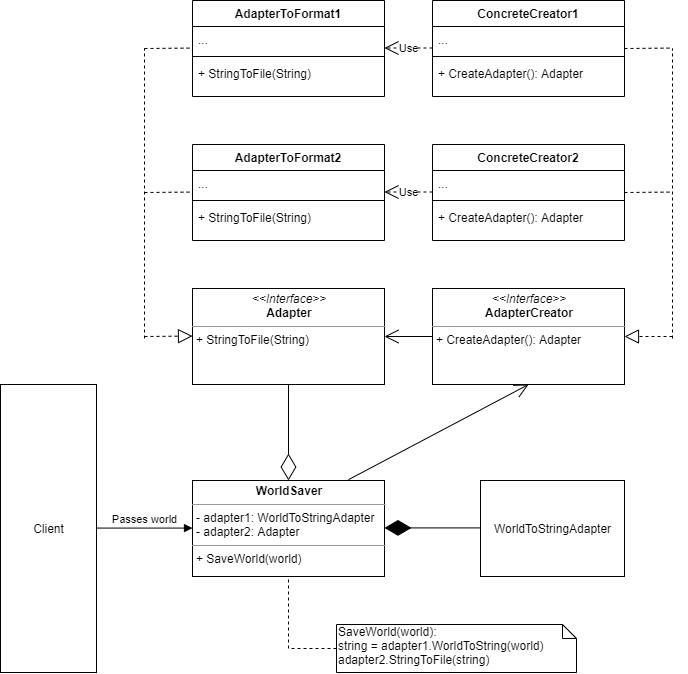
\includegraphics[scale=0.7]{uml}

\end{itemize}
}
\end{document}
